
\section{RESULTS}
\label{sec:results}

For the subsequent analyses, we obtained data for each parameter set by running the simulation for ten trials. Information about each student was recorded for every year of the 
simulation, and for each piece of anlaysis, we extracted the variable of interest by transforming this output into two vectors: one documenting the white students and another documenting the minority students. Each element of the vectors corresponds to the parameter of interest for one student. Often, this is the proportion of that individual's friends which are 
minorities, but on occasion we were interested in other variables. To prevent duplicates in the data, since a student who attended the college for four years would be included in the file four 
times, we considered only the data that was obtained during a student's senior year. With regards to friendship proportions, it is important to note 
that having no minority friends when you have some number of friends is potentially much different from having no 
minority friends when you have no friends in general. So, we also omitted the data where a student had zero total friends in the case where vectors represent proportions.
After creating a vector for each trial run, we concatenated the ten vectors. The resultant vectors were around 160,000 in 
length for the white data and around 40,000 in length for the minority data.

For the vector comparisons, we chose to use the Wilcoxon rank test (as opposed
to the more common Student's t-test) because our data is decidedly non-normal.
Figure 1 illustrates this fact by using the proportional data as an example. A
histogram of all proportional data for one set of ten trials (both white and
minority data included) is most closely modeled by the beta distribution
instead of a normal distribution. dA Q-Q plot shows evidence of
non-normality). We use the standard $\alpha=0.05$ rejection value for $p$.

\begin{figure}[ht]
  \centering
    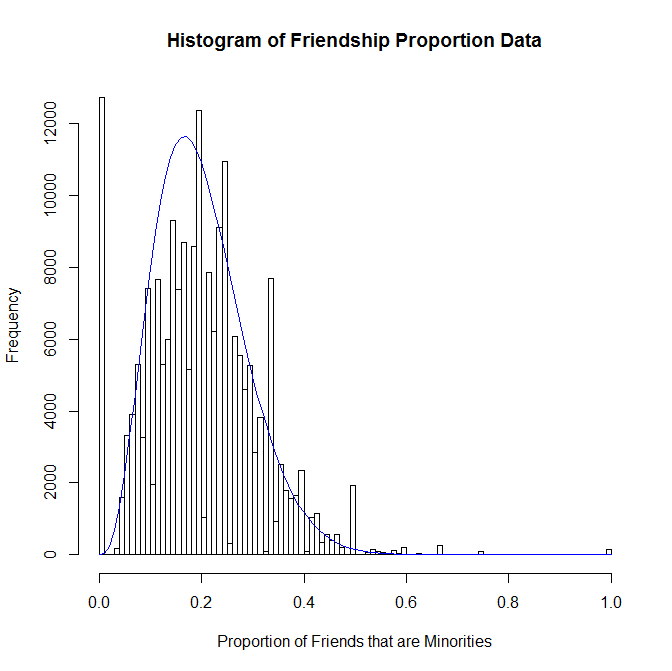
\includegraphics[width=0.5\textwidth]{histogramProportionData.png}
      \caption{A histogram of the proportional data compared to the Beta distribution.}
\end{figure}

\subsection{Simulation Verification}

%\begin{figure}[h]
%  \centering
%    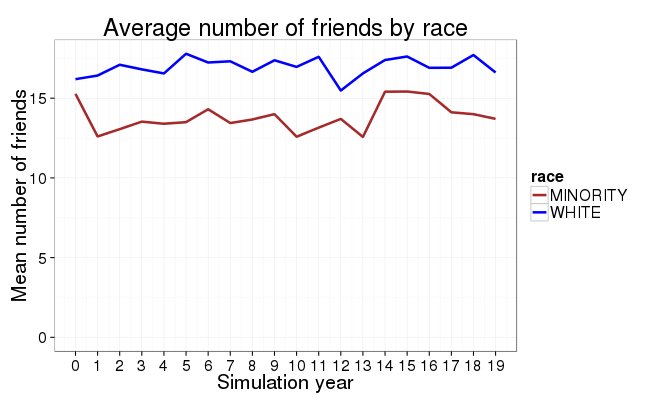
\includegraphics[width=0.5\textwidth]{avgNumberOfFriendsFromCaladan.png}
%      \caption{The average number of friends students possessed for one run of the simulation.}
%\end{figure}
First, it is important to inspect the data of the average number of friends held by minorities and whites across the years 
in the simulation. Note that for any $w_r\neq 0$, minorities had fewer friends on average than whites, regardless of other parameter settings. 
The following table shows the average number of friends held by each of the two races, with the associated $p$-value used to determine if 
the difference is significant.\\

\begin{center}
\begin{tabular}{|c|c|c|c|}
\hline
$w_r$ & Number of Friends: White & Number of Friends: Minority & $p$-value\\
\hline
0 & 15.66 & 15.73 & 0.0784\\
10 & 15.54 & 14.15 & $<2.2\times 10^{-16}$\\
20 & 15.49 & 12.97 & $<2.2\times 10^{-16}$\\
100 & 15.43 & 7.90 & $<2.2\times 10^{-16}$\\
\hline
\end{tabular}
\end{center}~~\\

That is, if race matters even slightly to the students in the simulation, then minorities will form fewer relationships. When race is not a factor in 
friendship formation, the races have an approximately equal average number of friends, as expected. Additionally, the number of friends held by whites 
does not vary for varying $w_r$, indicating that $w_r$ does not directly impact their ability to form and maintain relationships.

%%By creating stacked histograms of the racial composition of each group,
%We observed that the composition of groups at the null 
%race weight matched the expected composition, which was based on the population composition, more closely than any of the 
%nonzero race weights. As race weight increased, the observed group composition grew farther from that which was expected. In 
%fact, at the most extremely high values of race weight, an increasing proportion of the groups consisted only of white 
%students, as minorities lose affinity towards many groups, and thus can neither join nor remain in them.

%We used boxplots to track and display the frequency of perceived similarity levels whenever two students encountered each other.
For $w_r=0$, students participating in interracial encounters experienced the same perceived similarity levels as students involved in same-race encounters. For higher values of 
$w_r$, the homogeneous race interactions had similarity values that remained at approximately the same level. Meanwhile, the perceived similarity of heterogeneous race interactions 
creeped lower.
\begin{figure}
\begin{subfigure}{.5\textwidth}
  \centering
    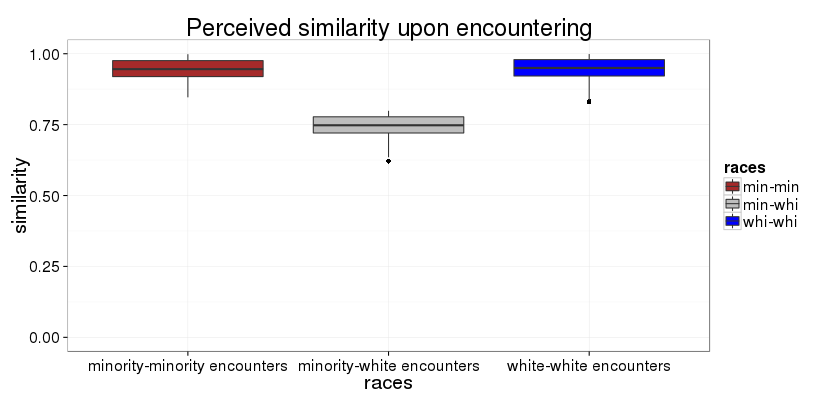
\includegraphics[width=1.2\textwidth]{similarityBoxplots20.png}
      \caption{Perceived similarity.}
\end{subfigure}
\begin{subfigure}{.5\textwidth}
    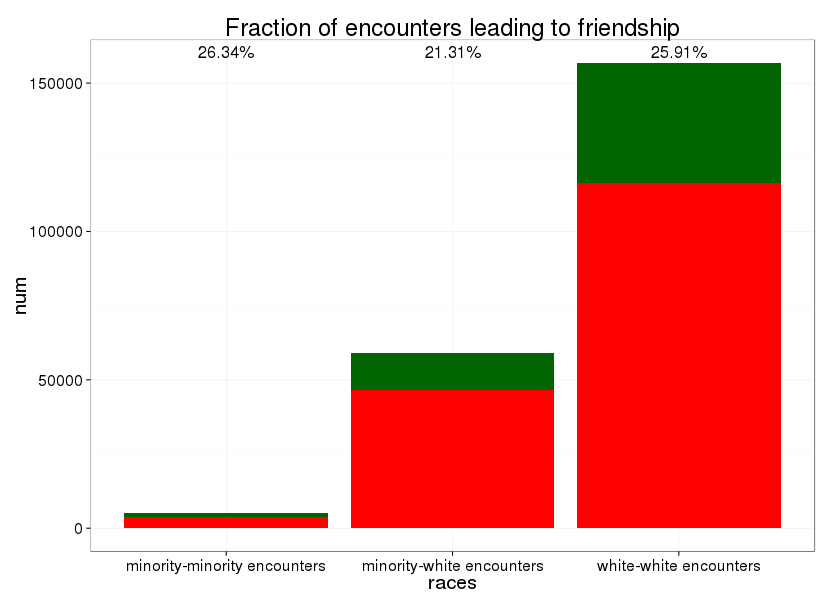
\includegraphics[width=\textwidth]{encountersGraph20.png}
      \caption{Fraction of encounters leading to friendship.}
\end{subfigure}
\caption{Perceived similarity and encounters for $w_r=20$.}
\end{figure}
Because of this, homogeneous encounters resulted in friendship slightly more 
often (with respect to a percentage) than heterogeneous encounters as $w_r$ was given positive value. As the importance of race increased, the proportion 
of heterogeneous encounters which resulted in friendship expectedly decreased. However, the proportion of homogeneous encounters 
which resulted in friendship stayed approximately the same.

\subsection{Discoveries}

After preliminary analyses utilizing various graphs, we proceeded to analyze the data in a more concrete manner. For the following observations, we 
choose to use the proportional friendship data.

%The data generated from race weight being set to 0 was used as our baseline reference 
%for purely integrated data. So, any comparion of data to this baseline reference that was insignificant could be called integrated. The data generated 
%from race weight equalling 100 was considered to be the extremely segregated reference point. Of course, race weight is unbounded, and it would 
%be impossible to find ``the absolute" maximum race weight to case 100\% segregation. We decided that at level 100, race weight is high enough 
%to be deemed extreme segregation. So, any comparison of data to this reference point that was insignificant could be called extremely integrated.

%Some weird results from this so I won't consider it for now

First, we generate a set of vectors for several values of $w_r$. A second set of vectors was generated using the same parameter sets as the first, but with the 
exception that we have ``turned on" a policy. An inactive policy, one whose parameter was previously zero, was set to have some nonzero parameter. Primarily, 
we investigated the potential effects of setting the parameter for {\bf OrientationGroups}, $n_{f_0}$, to five. We then 
determine if the policy had an effect by performing a Wilcoxon rank test on the sets of vectors - whites when policy is off versus whites when policy is on, and minorities when policy is off 
versus minorities when policy is on - to determine whether or not the policy had a distinguishable effect on the population.

For $w_r=0$, {\bf OrientationGroups} does not demonstrate any significant effect on the population. This policy also did not have an effect $w_r=1$, leaving 
the campus still as segregated as it was before the policy was implemented. These results were repeated again when $w_r$ was set to 10. However, when $w_r$ was increased to 20, the 
white population did experience a significant change after {\bf OrientationGroups} came ``on." Finally, for the extreme setting of $w_r=100$, {\bf OrientationGroups} again had a significant effect on the white data. To summarize, we discovered that below $w_r=20$, the policy had no effect. However, at this level and above, the policy did begin to influence the friendships being made by the Students. We also briefly investigated the effects of using $n_{f_0}=10$. When $w_r=1$, we continued to demonstrate the policy had a significant effect on the proportion of minority friends held by white students.

It may now be important to note that, while the next natural question may be about how the mean proportions changed, we are purposefully not reporting the mean values here. The mean is 
not a sufficient statistic for the beta distribution. That is, the information held in a distribution of this type is not adequately captured by reporting the mean, as it could be for a noraml distribution. To add, the values for the means are misleading. Even between statistically significant vectors, the difference in the means may be arbitrarily small to the naked eye. In fact, the alternative hypothesis for the Wilcoxon test is not that the means are equal, as in the Student's t-test, but instead is that the true location shift is not zero. Therefore, two statistically significant vectors may have the same or similar means, but come from two very different beta distributions with differing shape parameters and location shift not equal to zero. While this may be difficult to interpret within this context, the important conclusion is that the policy has been verified to have a tangible effect on the relationships formed by Students.


%The actual difference may 
%be unexpected: The policy caused the mean proportion of minority friends held by whites to \emph{decrease}, from 0.1646 to 0.1634. This is evidence that the policy actually caused higher segregation for whites. However, the positive result is that the mean proportion of minority friends held by minorities also decreased, from 0.2215 to 0.2201. This means that, on 
%average, minorities had a higher percentage of their friendships form with whites, improving the integration from their direction. 


%I left out that there was a non-significant effect on the minority data where the mean
%actually went up, so it's almost like the policy made things worse

%If a minority has fewer minority friends, they have more white friends, which means they experience more
%integration. Does that really help them at all? If I'm a minority, am I better off under a policy that causes me
%to have more white friends than I would have been otherwise? Or would it not be as much of an improvement as if I just had
%more friends in general? Or, would I feel more accepted if I could make lots of friends with people of my own race? Is the
%end game to make whites have more minority friends, or to make minorities have more white friends? Which is truly the most
%beneficial in terms of making minorities feel more accepted? Stephen?

%I could see the argument for "minorities having more friends that are white" being beneficial from the viewpoint that
%then they may not feel as threatened by other whites they encounter (may feel more at home/relaxed) as well as that the 
%spread of ideas due to interaction with people who are different is increased.

Finally, we momentarily examined the effects of using a different policy - {\bf InitialMixedRaceDyads} - on the 
populations. We set $n_{d_0}=10$, a value which is relatively high given the average total number of friendships (see table). At $w_r=1$, the policy had an effect on both races in the population. When this was repeated for $w_r=20$, the policy appears to have had no effect. It may be that even at a relatively low value for the importance of race, the policy is already not strong enough to overcome the perceived barrier.
